\chapter{骨骼与肌肉}\label{ch:g3:bones-and-muscles}

跳起并落地：你体内刚刚有一台完美的
机器在运转。坚硬的“杆”撑起你的身形，铰链让你的腿能屈伸、弹起，
数百个小“马达”在需要时准确发力。
骨是“杆”，\omterm{def:g1:my-body:joint}{关节}是“铰链”，
\omterm{def:g3:bones-and-muscles:muscle}{肌肉}是“马达”——身体为一生中的每一次运动
准备的全部装备。

\section{骨骼}

\begin{definition}[骨骼与骨]\label{def:g3:bones-and-muscles:skeleton}
人体内的\emph{骨骼}\index{骨骼}是由约 $200$ 块
\emph{骨}\index{骨}组成的支架。主要部分有：
\begin{itemize}
  \item \emph{颅骨}\index{颅骨}，即由坚硬的骨构成的“头盔”，
        包在脑的外面；
  \item \emph{脊柱}\index{脊柱}，可以弯曲的一根柱子，
        由许多小骨从颈部一直叠到髋部，
        支撑着躯干直立；
  \item \emph{肋骨}\index{肋骨}，弯曲的骨围成一个笼子，
        保护心脏与肺；
  \item \emph{\omterm{def:g1:my-body:parts}{四肢}骨}：手臂和腿中的长骨——
        大腿骨是全身最长的骨。
\end{itemize}
\end{definition}

\begin{omfigure}
\begin{tikzpicture}
  \node[anchor=south west, inner sep=0] (img) at (0,0)
    {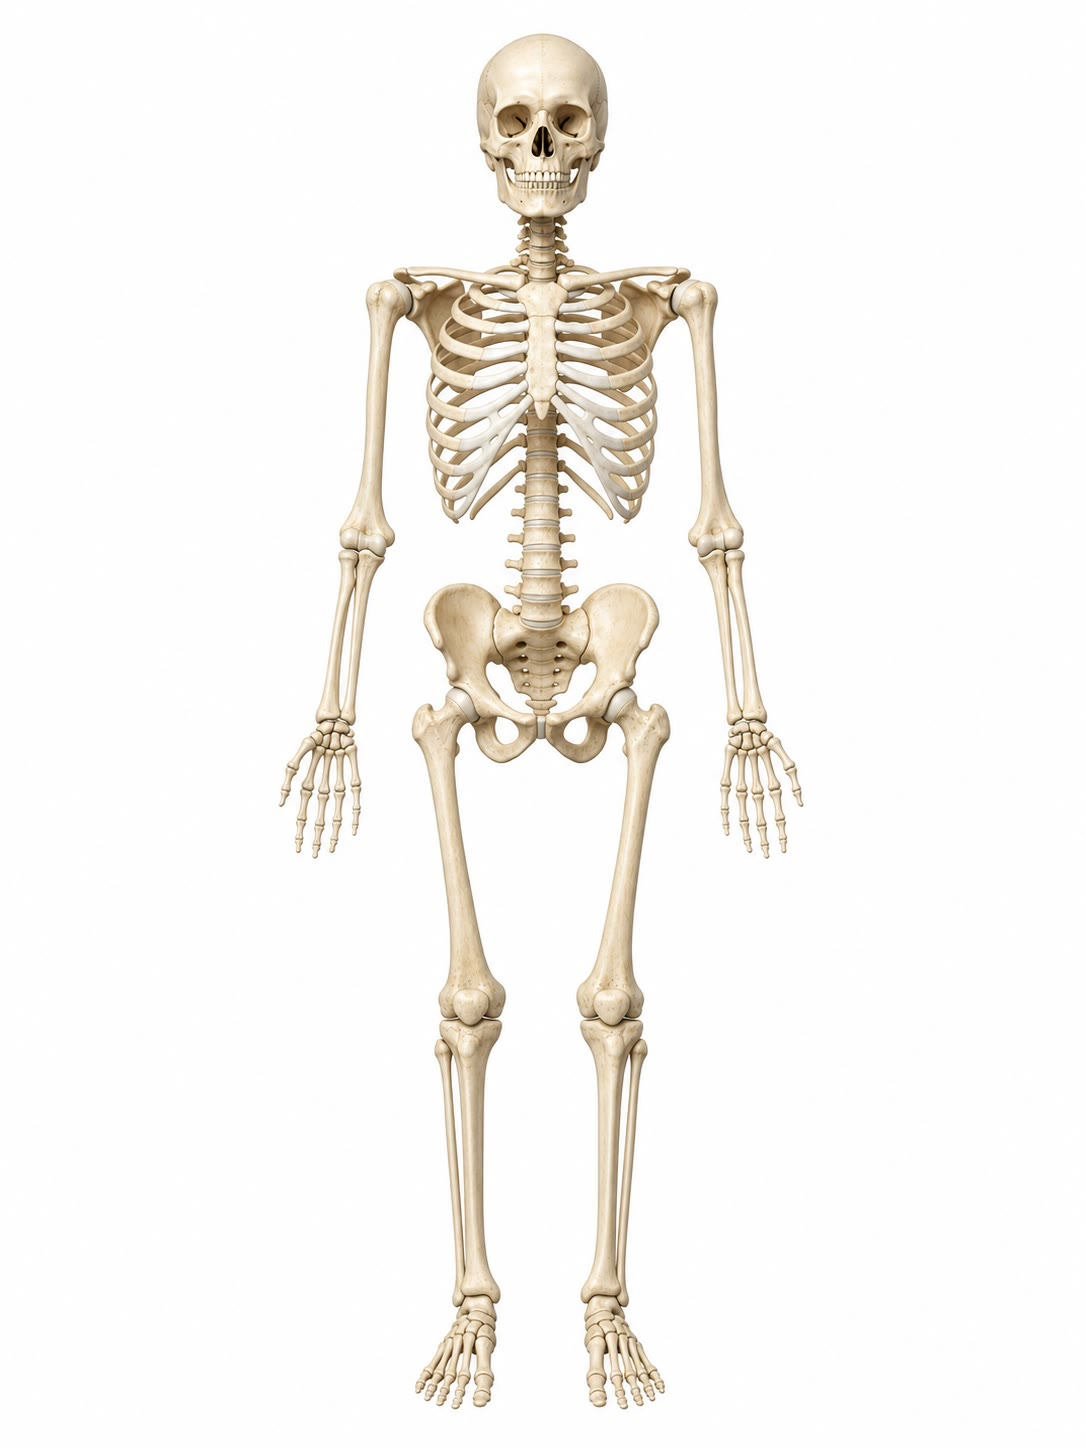
\includegraphics[width=0.46\linewidth]{images/book1/ai/fig-skeleton.jpg}};
  \begin{scope}[x={(img.south east)}, y={(img.north west)},
      every node/.style={font=\small}]
    \draw[omDef, thick] (0.56,0.93) -- (0.72,0.95) node[right] {颅骨};
    \draw[omDef, thick] (0.40,0.73) -- (0.20,0.82)
      node[above, align=center] {肋骨：围护心脏 \\ 与肺};
    \draw[omDef, thick] (0.52,0.56) -- (0.72,0.60)
      node[right, align=left] {脊柱：叠起的 \\ 小骨};
    \draw[omDef, thick] (0.60,0.36) -- (0.76,0.38) node[right] {大腿骨};
    \draw[omThm, thick] (0.335,0.615) circle (0.022);
    \draw[omThm, thick] (0.445,0.265) circle (0.022);
    \draw[omThm, thick] (0.425,0.265) -- (0.20,0.22)
      node[left, align=center, omThm] {关节（红色）：\\ 两骨相接之处};
  \end{scope}
\end{tikzpicture}

{\small \omterm{def:g3:bones-and-muscles:skeleton}{骨骼}的布局：头盔、\omterm{def:g3:bones-and-muscles:skeleton}{脊柱}、胸笼，以及在\omterm{def:g1:my-body:joint}{关节}处
相接的\omterm{def:g1:my-body:parts}{四肢}长骨。}
\end{omfigure}

\begin{example}[摸一摸你的骨架]\label{ex:g3:bones-and-muscles:feel}
不用 X 光：轻轻按一按，\omterm{def:g3:bones-and-muscles:skeleton}{骨骼}就会“告诉”你。指\omterm{def:g1:my-body:joint}{关节}；
胫骨前缘；沿背部正中一串小小的凸起——
\omterm{def:g3:bones-and-muscles:skeleton}{脊柱}，一节接一节的小骨；
还有\omterm{def:g3:bones-and-muscles:skeleton}{肋骨}，用手指就能数出来。骨架就在
\omterm{def:g1:the-five-senses:sense}{皮肤}下面。
\end{example}

\begin{remark}[外硬内活]\label{rem:g3:bones-and-muscles:alive}
骨并不是像粉笔那样的死物：它是活的，靠血液供养，
随着你的成长而生长，还能自我修复。
手臂骨折后打了石膏，之所以能愈合，
是因为骨本身在慢慢修补断口。粉笔可做不到这一点。
\end{remark}

\begin{omfigure}
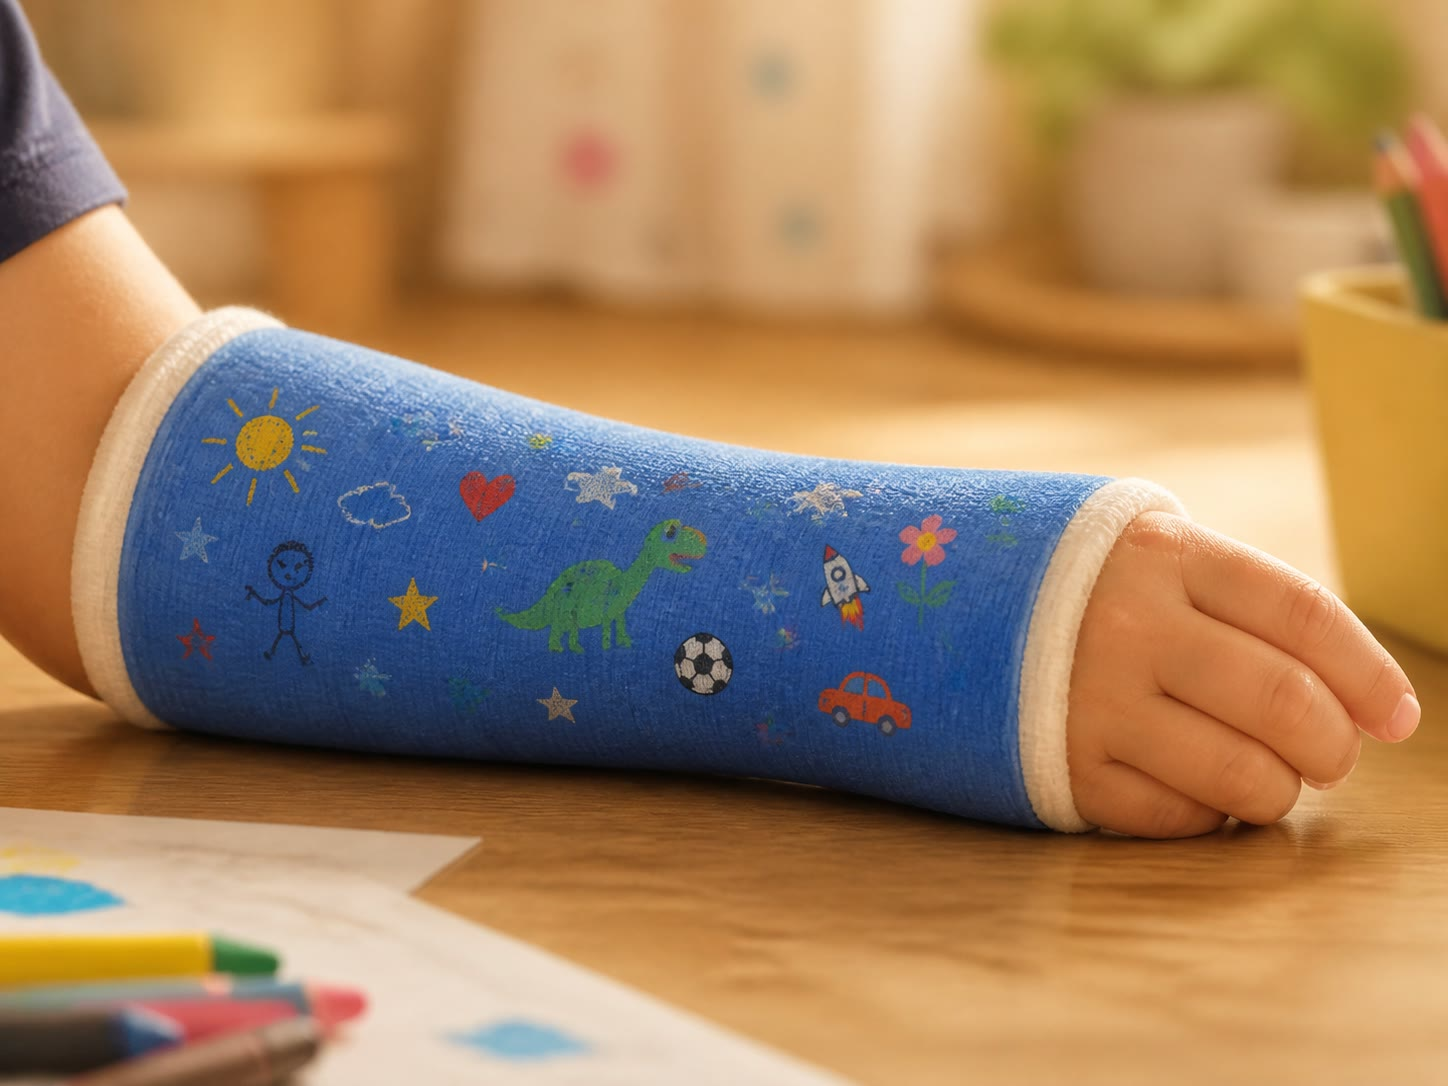
\includegraphics[width=0.56\linewidth]{images/book1/ai/g3-bones-cast.jpg}

{\small 彩绘石膏固定着手臂，其中的活骨
正在悄悄地修复自己。}
\end{omfigure}

\section{关节：骨架弯曲之处}

\begin{proposition}[坚硬的杆，弯曲之处]\label{prop:g3:bones-and-muscles:joints}
骨本身从不弯曲——弯了的骨就是断了的骨。
身体的一切弯曲都发生在
\emph{关节}\index{关节}处，即两骨相接之处：肩、
肘、腕、髋、膝、踝，以及\omterm{def:g3:bones-and-muscles:skeleton}{脊柱}中许多小
\omterm{def:g1:my-body:joint}{关节}，它们的小幅弯曲累积起来，使背部柔韧。
\end{proposition}
\admitted

\begin{example}[脊柱的窍门]\label{ex:g3:bones-and-muscles:spinetrick}
背上没有哪一块骨能卷起来——但你能向前滚动
几乎卷成一个球。\omterm{def:g3:bones-and-muscles:skeleton}{脊柱}由超过
$20$ 块小骨构成，每一块都只能相对于相邻的骨转动几度：
许多小弯曲合成一个大弯曲。这也是为什么
搬重物时应当弯膝而不是弯腰——膝
适合大幅度弯折，\omterm{def:g3:bones-and-muscles:skeleton}{脊柱}则适合轻柔的弯曲。
\end{example}

\section{肌肉：运动的动力}

\begin{definition}[肌肉]\label{def:g3:bones-and-muscles:muscle}
\emph{肌肉}\index{肌肉}是附着在骨上的一台肉质的
“马达”。肌肉能\emph{收缩}\index{收缩}——缩短、
变粗，收缩时它会\emph{拉动}所附着的
骨。肌肉只能拉，不能推。
\end{definition}

\begin{proposition}[成对工作]\label{prop:g3:bones-and-muscles:pairs}
既然\omterm{def:g3:bones-and-muscles:muscle}{肌肉}只能拉，要让\omterm{def:g1:my-body:joint}{关节}双向运动，就需要一
\emph{对}\omterm{def:g3:bones-and-muscles:muscle}{肌肉}：手臂前面的一块\omterm{def:g3:bones-and-muscles:muscle}{肌肉}使肘弯曲，它的
后面的“搭档”使肘伸直；两者轮流，一块放松时，另一块
拉动。身体中几乎每个\omterm{def:g1:my-body:joint}{关节}都由这样的\omterm{def:g3:bones-and-muscles:muscle}{肌肉}对来运动。
\end{proposition}
\admitted

\begin{omfigure}
\begin{tikzpicture}
  \node[anchor=south west, inner sep=0] (img) at (0,0)
    {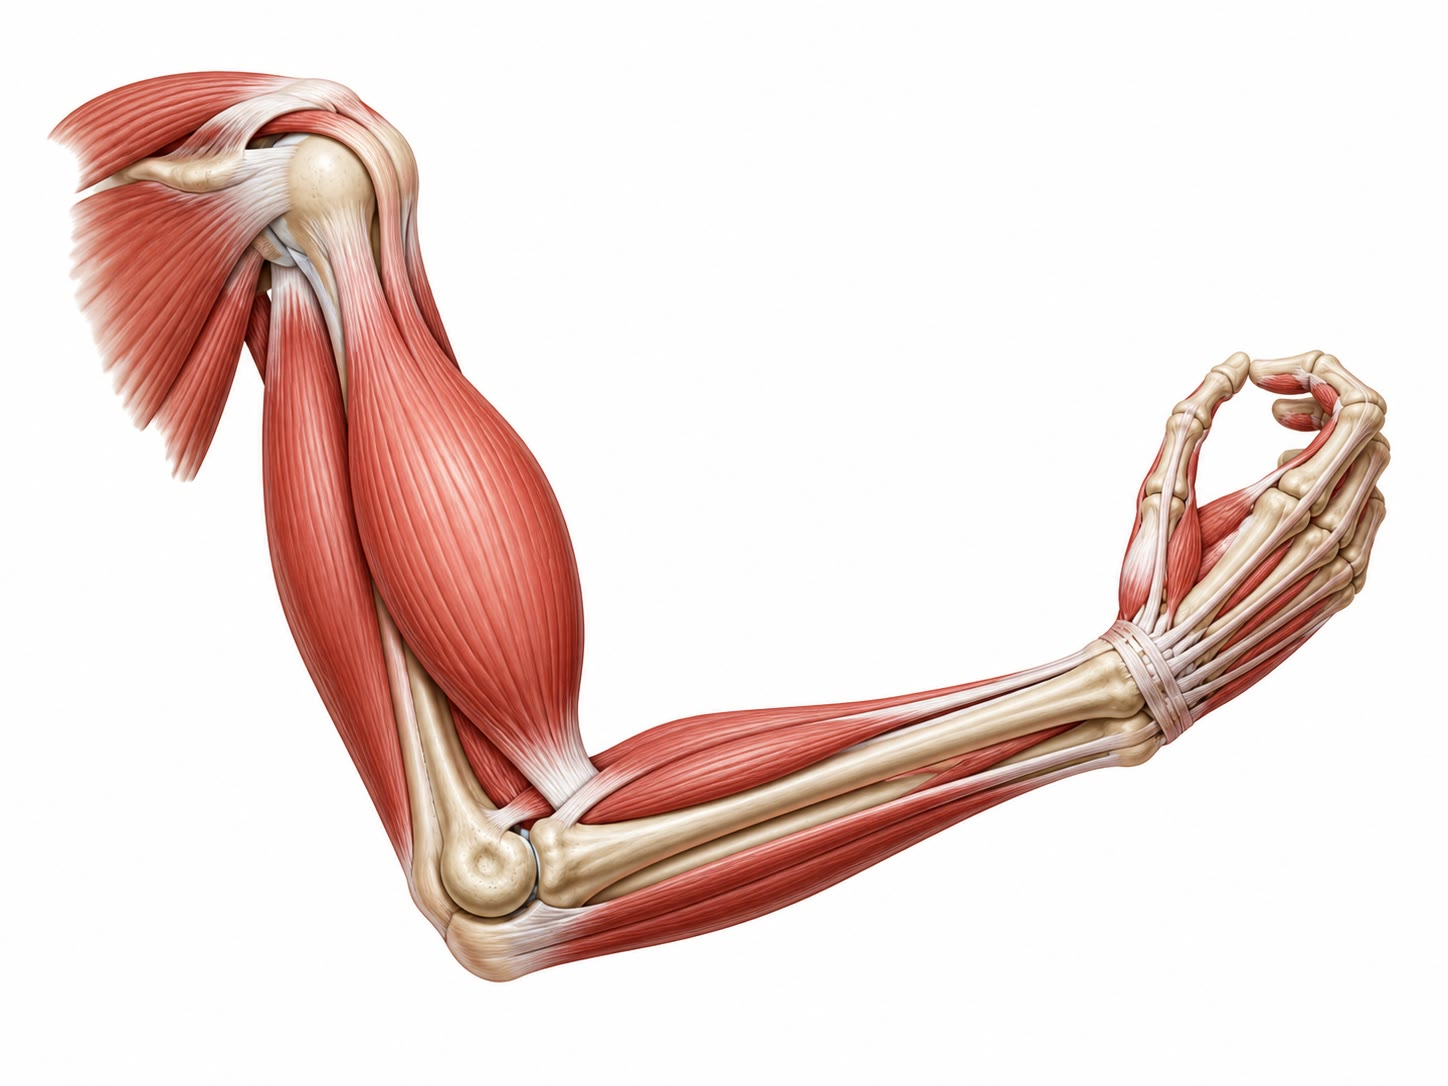
\includegraphics[width=0.62\linewidth]{images/book1/ai/fig-arm-muscles.jpg}};
  \begin{scope}[x={(img.south east)}, y={(img.north west)},
      every node/.style={font=\small}]
    \draw[omThm, thick] (0.42,0.58) -- (0.58,0.78)
      node[right, align=left, omThm]
      {前面鼓起的肌肉：\\ 它收缩并拉动};
    \draw[omDef, thick] (0.23,0.46) -- (0.14,0.22)
      node[below, align=center, omDef]
      {后面的肌肉 \\ 这一对中的另一块，放松};
  \end{scope}
\end{tikzpicture}

{\small 屈肘时，这一对\omterm{def:g3:bones-and-muscles:muscle}{肌肉}中前面的那块鼓起，
缩短并把前臂向上拉，后面的同伴则
放松。伸直手臂时，两者角色互换。}
\end{omfigure}

\begin{example}[感受这一对肌肉的工作]\label{ex:g3:bones-and-muscles:pair}
用另一只手握住上臂，慢慢弯曲
手肘：前面的\omterm{def:g3:bones-and-muscles:muscle}{肌肉}会鼓起变硬——它正在\omterm{def:g3:bones-and-muscles:muscle}{收缩}。
现在伸直手臂：前面的\omterm{def:g3:bones-and-muscles:muscle}{肌肉}变软，
而手臂后面的同伴则会绷紧。你刚刚感受到的
正是\cref{prop:g3:bones-and-muscles:pairs}中的现象。
\end{example}

\begin{method}[爱护骨骼和肌肉]\label{met:g3:bones-and-muscles:care}
\begin{enumerate}
  \item 每天都要运动——\omterm{def:g3:bones-and-muscles:skeleton}{骨骼}会变得更结实，\omterm{def:g3:bones-and-muscles:muscle}{肌肉}也一样，
        越用越强壮；
  \item 多吃“建造者”食物：奶制品有益\omterm{def:g3:bones-and-muscles:skeleton}{骨骼}，还要
        饮食多样（见\cref{ch:g2:teeth-and-eating-well}）；
  \item 剧烈运动前先热身，使\omterm{def:g3:bones-and-muscles:muscle}{肌肉}被拉伸而
        不是被撕裂；
  \item 搬重物时屈膝、保持背部挺直；
  \item 在容易摔倒的地方戴头盔、穿护具：\omterm{def:g3:bones-and-muscles:skeleton}{骨骼}会修复，
        但修复得很慢。
\end{enumerate}
\end{method}

\section{练习}

\begin{exercise}[$\star$]\label{exo:g3:bones-and-muscles:1}
说出\cref{def:g3:bones-and-muscles:skeleton}中
\omterm{def:g3:bones-and-muscles:skeleton}{骨骼}的四个部分，以及各部分
分别保护或支撑什么。
\end{exercise}

\begin{exercise}[$\star$]\label{exo:g3:bones-and-muscles:2}
\omterm{def:g3:bones-and-muscles:skeleton}{骨骼}大约有多少块骨头？哪一块最长？
\end{exercise}

\begin{exercise}[$\star$]\label{exo:g3:bones-and-muscles:3}
骨头能弯曲吗？身体的弯曲都发生在哪里？
\end{exercise}

\begin{exercise}[$\star$]\label{exo:g3:bones-and-muscles:4}
\omterm{def:g3:bones-and-muscles:skeleton}{脊柱}能够弯曲，尽管它的每块骨头都不能弯曲。
请解释其中的诀窍。
\end{exercise}

\begin{exercise}[$\star$]\label{exo:g3:bones-and-muscles:5}
\omterm{def:g3:bones-and-muscles:muscle}{肌肉}\omterm{def:g3:bones-and-muscles:muscle}{收缩}时做什么？还有，
\omterm{def:g3:bones-and-muscles:muscle}{肌肉}永远不能做什么？
\end{exercise}

\begin{exercise}[$\star$]\label{exo:g3:bones-and-muscles:6}
为什么屈伸肘部需要两块\omterm{def:g3:bones-and-muscles:muscle}{肌肉}？
请说明在每个时刻，每块\omterm{def:g3:bones-and-muscles:muscle}{肌肉}各自做什么。
\end{exercise}

\begin{exercise}[$\star$]\label{exo:g3:bones-and-muscles:7}
打了石膏的手臂是怎样愈合的？这说明\omterm{def:g3:bones-and-muscles:skeleton}{骨骼}
有什么特点？请结合\cref{rem:g3:bones-and-muscles:alive}作答。
\end{exercise}

\begin{exercise}[$\star$]\label{exo:g3:bones-and-muscles:8}
动手试一试：在自己的手臂上做\cref{ex:g3:bones-and-muscles:pair}中
的握紧测试。描述弯曲手臂时，手臂前面
有什么变化，伸直手臂时又有什么变化。
\end{exercise}

\begin{exercise}[$\star\star$]\label{exo:g3:bones-and-muscles:9}
大人为什么说“搬东西要用膝盖发力，而不要用
背”？请用\cref{ex:g3:bones-and-muscles:spinetrick}作答。
\end{exercise}

\begin{exercise}[$\star\star$]\label{exo:g3:bones-and-muscles:10}
提线木偶可以被操纵着挥手：每根线只能
\emph{拉}动它的手臂向一个方向。这与\omterm{def:g3:bones-and-muscles:muscle}{肌肉}的处境
完全相同吗？木偶操纵者又如何应对这一问题？
请与\cref{prop:g3:bones-and-muscles:pairs}作比较。
\end{exercise}
